\section{Downloading and parsing indices}

As can be seen in figure \ref{fig:overview}, the first step of the process is to download data from Common Crawl. This requires functions that will parse the Common Crawl indices and gather the data that corresponds to these indices. 

\begin{figure}[H]
\centering
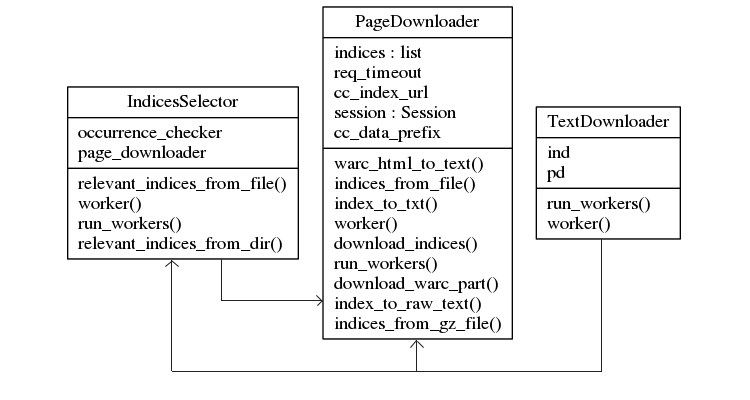
\includegraphics[width=0.8\textwidth]{gathering_class}
\caption{Diagram of downloading and parsing classes}
\label{fig:gathering_class}
\end{figure}

The parsing of indices and downloading the data depends on the IndicesSelector and PageDownloader class, methods from these classes are called by the TextDownloader, as can be seen in figure \ref{fig:gathering_class}. The classes contain workers, these workers can be run  using the \textit{run\_workers()} method which will utilise Python multiprocessing\footnote{\url{https://docs.python.org/3.5/library/multiprocessing.html}} to run workers in parallel. Running these workers in parallel speeds up the downloading of data \unsure{maybe other word instead of data?} and parsing of Common Crawl indices.

The first step in parsing the Common Crawl indices is filtering out the indices that have a HTTP Status Code \footnote{\url{https://www.w3.org/Protocols/rfc2616/rfc2616-sec10.html}} other than 200, as only these indices with these HTTP Status Code would be useful. 

\begin{lstlisting}[language=Python, caption=Initial implementation, label={lst:initial}]
def _useful_responsecode(self, index):
# Check responsecode of index to determine if it's useful to download
# the part. HTTP 200 is useful, other than 200 will be discarded.
    if index:
        return True if int(index['status']) == 200 else False
    return False

def _clean_indices(self, indices):
    # Removes useless entries with status code other than 200
    for index in indices:
        if not self._useful_responsecode(index):
    indices.remove(index)
\end{lstlisting}

At first a simple implementation was used as can be seen in listing \ref{lst:initial}. However, a remove operation on a list in Python has a time complexity of O(n), the implementation of \textit{clean\_indices()} loops over all indices and removes it if it has status other than 200, which meant that this function had a complexity of $O(n^2)$. To improve this, a regular expression to search the string for the status before parsing to JSON is ued. This way, the list will never contain any indices with a HTTP Status Code other than 200 as the function will is called in a list-comprehension. This resulted in a speedup of about 5.6 times compared to the $O(n^2)$ method.

\begin{lstlisting}[language=Python, caption=Regex solution]
def _useful_str_responsecode(string):
    if string:
        return int(re.search('\"status\": \"(\w+)\",', string)
                   .group(1)) == 200
\end{lstlisting}

While parsing the index the memory footprint of the indices is also reduced, with use of the method from listing \ref{lst:memory}. Parsing every key of the index to JSON meant the resulting JSON dict was 480 bytes, where the size of the stripped index was 288 bytes. The size of the objects was determined using the Python built-in \textit{sys.getsizeof()} method. 

\begin{lstlisting}[language=Python, caption=Reducing memory footprint, label={lst:memory}]
def _remove_keys(json_dict):
# Strip all key-value pairs other than digest, length, offset & name
    return {k: v for k, v in json_dict.items()
            if k in ['digest', 'length', 'offset', 'filename']}
\end{lstlisting}
